\begin{center}
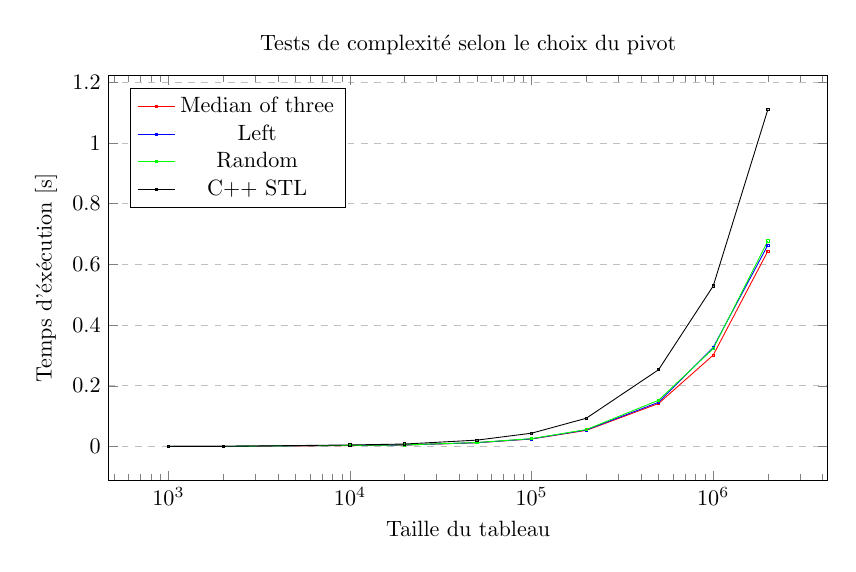
\begin{tikzpicture}[scale=0.8]
\begin{axis}[
    title={Tests de complexité selon le choix du pivot},
    xlabel={Taille du tableau},
    ylabel={Temps d'éxécution [s]},
    legend pos=north west,
    ymajorgrids=true,
    grid style=dashed,
	xmode=log,
	width=13cm,
	height=8cm
]
 
\addplot[color=red, mark=square, mark size=0.5]
    coordinates {
		(1000,0.000381)(2000,0.000795)(10000,0.003054)(20000,0.005002)(50000,0.012493)(100000,0.025005)(200000,0.053209)(500000,0.141692)(1000000,0.301091)(2000000,0.643868)
	};

\addplot[color=blue, mark=square, mark size=0.5]
	coordinates {
		(1000,0.000406)(2000,0.000901)(10000,0.003676)(20000,0.005117)(50000,0.012768)(100000,0.025317)(200000,0.054655)(500000,0.14572)(1000000,0.326452)(2000000,0.663702)
};

\addplot[color=green, mark=square, mark size=0.5]
	coordinates {
		(1000,0.000438)(2000,0.000881)(10000,0.003754)(20000,0.005347)(50000,0.013282)(100000,0.026137)(200000,0.055889)(500000,0.152488)(1000000,0.322487)(2000000,0.677414)
};

\addplot[color=black, mark=square, mark size=0.5]
	coordinates {
		(1000,0.000316)(2000,0.000703)(10000,0.005228)(20000,0.008305)(50000,0.021153)(100000,0.043995)(200000,0.093181)(500000,0.252968)(1000000,0.528827)(2000000,1.110281) 
	};

\legend{Median of three,Left,Random, C++ STL} 
\end{axis}
\end{tikzpicture}
\end{center}
